\documentclass[sigconf,natbib=true,anonymous=true]{acmart}

\acmConference[CIKM '26]{The 35th ACM International Conference on Information and Knowledge Management}{November 7--11, 2026}{Rome, Italy}
\acmYear{2026}

\hypersetup{
    bookmarks=true,
    bookmarksopen=true,
    bookmarksnumbered=true,
    pdfborder={0 0 0},
    colorlinks=false,
    pdftitle={PMC: Build-Time Per-Modality Centroid Correction for Cross-Modal Binary-Quantized Retrieval},
    pdfauthor={Anonymous Author(s)},
    pdfsubject={CIKM 2026 Short Paper},
    pdfkeywords={cross-modal retrieval, modality gap, approximate nearest neighbor search, binary quantization}
}

\usepackage{algorithm}
\usepackage{algpseudocode}
\usepackage{booktabs}
\usepackage{amsmath}
\usepackage{graphicx}
\usepackage{subcaption}
\usepackage{flushend}
\usepackage{enumitem}
\usepackage{microtype}

\title{PMC: Build-Time Per-Modality Centroid Correction for Cross-Modal Binary-Quantized Retrieval}

\author{Anonymous Author(s)}
\affiliation{%
  \institution{Anonymous Institution}
}

\setlength{\textfloatsep}{2pt plus 1pt minus 1pt}
\setlength{\floatsep}{6pt plus 1pt minus 1pt}
\setlength{\intextsep}{4pt plus 2pt minus 2pt}
\setlength{\abovecaptionskip}{2pt}
\setlength{\belowcaptionskip}{1pt}
\setlength{\dbltextfloatsep}{2pt plus 1pt minus 1pt}
\setlength{\dblfloatsep}{4pt plus 2pt minus 2pt}
\setcounter{topnumber}{10}
\setcounter{dbltopnumber}{10}
\renewcommand{\topfraction}{0.95}
\renewcommand{\dbltopfraction}{0.95}
\renewcommand{\floatpagefraction}{0.7}
\renewcommand{\dblfloatpagefraction}{0.7}
\begin{document}

\setlength{\abovedisplayskip}{10pt plus 2pt minus 5pt}
\setlength{\belowdisplayskip}{10pt plus 2pt minus 5pt}

\begin{abstract}
Approximate nearest neighbor search is a core operator in large-scale retrieval, where vector quantization is widely used to reduce memory cost. Binary quantization methods encode each dimension as a single bit, but they assume queries and database vectors share a common centroid. This assumption fails in cross-modal retrieval, where each modality clusters around a different centroid, producing a modality gap that corrupts the centroid's dual role as inverted-file routing pivot and sign-bit decision boundary. We propose Per-Modality Centroid Correction (PMC), which shifts database vectors toward the query centroid at build time, rewriting routing and code boundaries at the source rather than merely adjusting queries at serving time. A selective variant confirms that concentrated gap energy in a few dimensions drives most recall loss. PMC adds no index memory or serving overhead; at $\alpha{=}1$, the correction is fully absorbed into the index with zero query-time cost. Experiments on five cross-modal benchmarks, three encoders, and four binary-quantized index types show gains over uncorrected and query-shifted baselines that scale with modality-gap magnitude, up to a 400M-vector deployment. Code: \url{https://anonymous.4open.science/r/PMC-CIKM}.
\end{abstract}


\begin{CCSXML}
<ccs2012>
<concept>
<concept_id>10002951.10003317.10003347.10003352</concept_id>
<concept_desc>Information systems~Multimedia and multimodal retrieval</concept_desc>
<concept_significance>500</concept_significance>
</concept>
<concept>
<concept_id>10002951.10003317.10003347.10003356</concept_id>
<concept_desc>Information systems~Search engine indexing</concept_desc>
<concept_significance>300</concept_significance>
</concept>
</ccs2012>
\end{CCSXML}

\ccsdesc[500]{Information systems~Multimedia and multimodal retrieval}
\ccsdesc[300]{Information systems~Search engine indexing}

\keywords{cross-modal retrieval, modality gap, approximate nearest neighbor search, binary quantization}

\maketitle

\section{Introduction}\label{sec:intro}

Multimodal foundation models such as CLIP~\cite{radford2021clip} and
ImageBind~\cite{girdhar2023imagebind} map heterogeneous signals (images,
text, audio) into a shared vector space for cross-modal vector similarity
search~\cite{jia2021align}. At deployment scale, storage becomes the
bottleneck: high-dimensional \texttt{float32} embeddings can require terabytes of RAM,
motivating approximate nearest neighbor (ANN) indexes that compress to a few bytes per
vector~\cite{jegou2011pq,gao2024rabitq}.\looseness=-1

Binary quantization (BQ) is the extreme compression point:
RaBitQ~\cite{gao2024rabitq} reaches $32\times$ compression by encoding each
dimension as one sign bit relative to the dataset centroid. Its production
adoption in Apache Lucene BBQ and extension to multi-bit
Extended-RaBitQ~\cite{gao2025extended} show BQ indexing is now
practically deployed.\looseness=-1

\begin{figure}[!t]
  \centering
  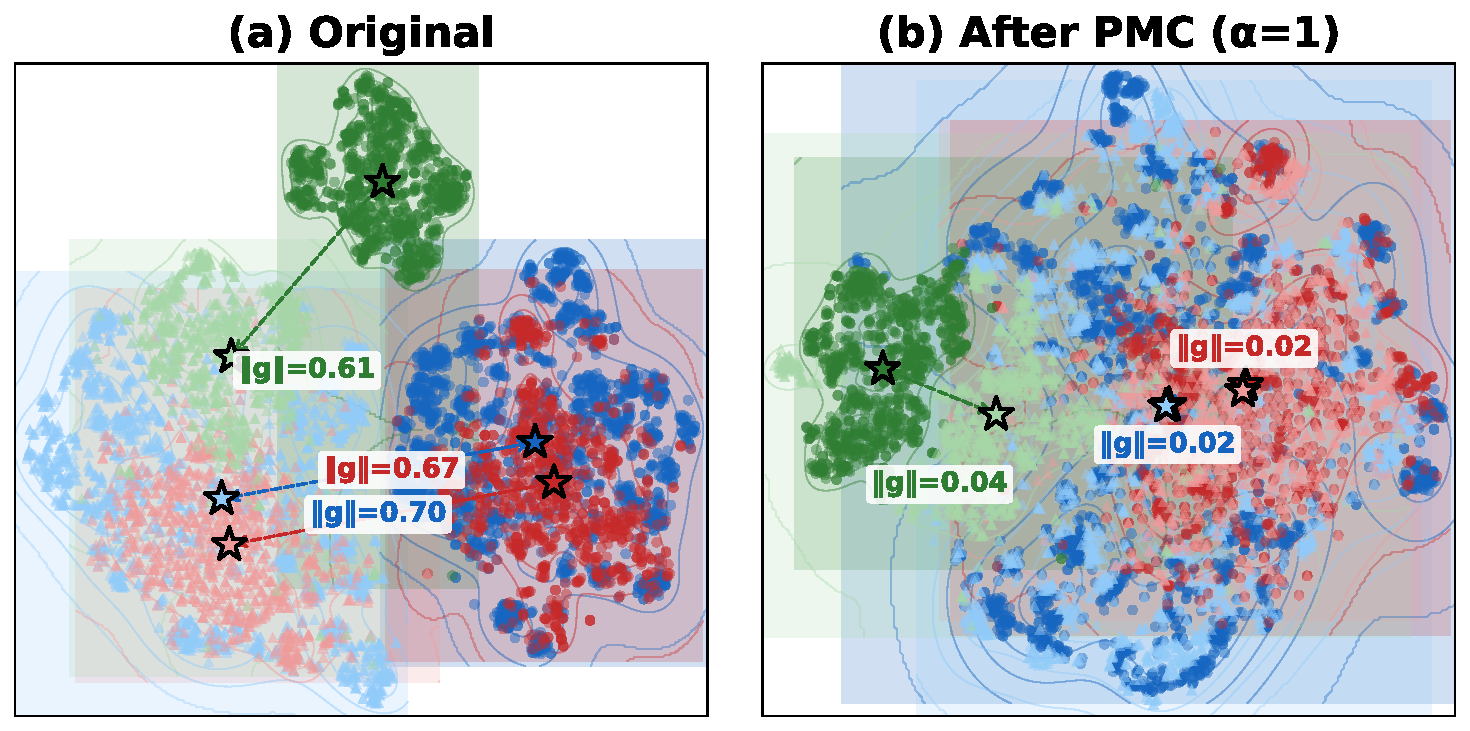
\includegraphics[width=\columnwidth]{figures/fig1_tsne.pdf}
  \Description{t-SNE visualization of ImageBind embeddings from three cross-modal datasets (MSCOCO, Flickr30K, Clotho) before and after PMC correction. Panel (a) shows separated modality clusters in the original space; panel (b) shows aligned clusters after PMC at alpha equals one.}
  \caption{t-SNE of ImageBind embeddings. (a)~Each modality forms a separate cluster. (b)~After PMC ($\alpha{=}1$), paired modalities overlap. Blue\,=\,MSCOCO, red\,=\,Flickr30K, green\,=\,Clotho; dark\,=\,DB, light\,=\,query.}\label{fig:modality-gap}
\end{figure}

{\emergencystretch=1em
These methods rely on a shared-centroid residual premise: queries and database
vectors are drawn from the same distribution and share a common centroid. Cross-modal
retrieval violates this assumption---\hspace{0pt}queries from one modality cluster around
a different centroid than the database vectors.\looseness=-1\par}

This \emph{modality gap}~\cite{liang2022mind} is particularly harmful to BQ
because the encoding $\mathrm{sign}(x_i - c_i)$ has \emph{zero
error margin}: the decision boundary passes exactly through the centroid,
and any systematic displacement causes structured bit corruption that
scales with gap magnitude (Figure~\ref{fig:modality-gap}); an oracle test confirms this: same-modality queries ($\|\mathbf{g}\|{=}0$) reach R@100$=$0.84 under RaBitQ, versus 0.57 for cross-modal queries ($\|\mathbf{g}\|{=}0.82$).
Prior work addresses cross-modal retrieval through graph
augmentation~\cite{chen2024roargraph,jaiswal2022ood}, encoder
fine-tuning~\cite{eslami2025alignclip}, or embedding-space
calibration~\cite{li2025grclip}, but none targets compressed ANN indexes
where centroid misalignment corrupts both Inverted File (IVF) routing and binary
codes.\looseness=-1

In this paper, we first analyze how the modality gap degrades BQ ANN indexes at two coupled stages---IVF routing and binary
code formation---and show that dimensions with concentrated gap energy
are most vulnerable to boundary crossing; a selective correction test
confirms that correcting only the highest-gap dimensions recovers most
of the gain.
Based on this analysis, we propose Per-Modality Centroid Correction
(PMC), a one-time build-time alignment that shifts database vectors
toward the query centroid before index construction. Unlike query-only
mean shift, which leaves IVF centroids and quantized codes misaligned,
PMC exploits the centroid's dual role as IVF routing pivot and sign-bit decision boundary, rewriting both at the source with no serving-time query transform and no additional index memory
(Figure~\ref{fig:pmc-overview}). We validate PMC across five cross-modal benchmarks including 407M-scale LAION, three multimodal encoders, and four BQ index types. Our contributions:
\begin{itemize}[nosep,leftmargin=*,topsep=0pt]
\item We show that the modality gap corrupts both IVF routing and binary codes, with recall loss scaling with gap magnitude.
\item We discover that this corruption concentrates in a few high-$|g_i|$ dimensions; a selective PMC variant correcting only those recovers most recall.
\item We propose PMC, a zero-cost build-time correction ($\alpha{=}1$) that realigns routing and codes via the centroid's dual role; ablation confirms DB-side over query-side correction.
\end{itemize}

\begin{figure}[t]
  \centering
  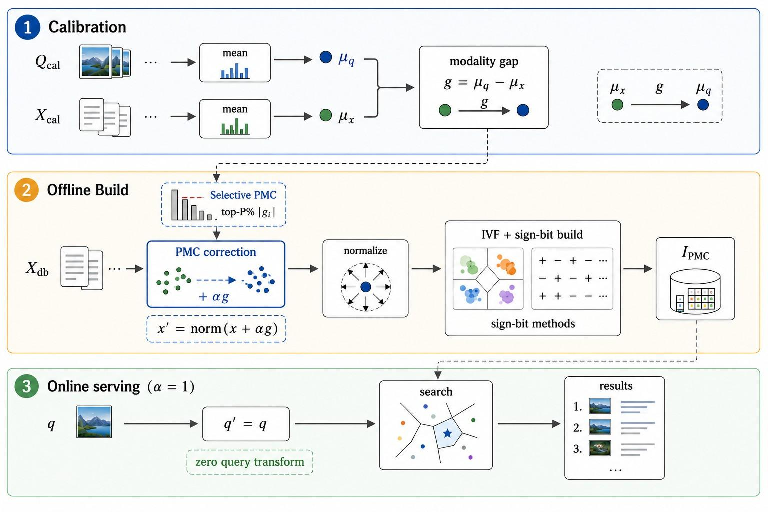
\includegraphics[width=\columnwidth]{figures/fig2_overview.pdf}
  \caption{PMC workflow: calibration estimates $\boldsymbol{\mu}_q$, $\boldsymbol{\mu}_x$, and $\mathbf{g}{=}\boldsymbol{\mu}_q-\boldsymbol{\mu}_x$; offline build shifts/normalizes database vectors before BQ index construction; at $\alpha{=}1$, online serving uses $\mathbf{q}'{=}\mathbf{q}$ and searches $\mathcal{I}_{\mathrm{PMC}}$.}
  \Description{Three-lane landscape PMC overview. Lane 1 (Calibration / Gap Estimation) takes calibration query and database samples, computes means mu-q and mu-x, and outputs the modality gap g equals mu-q minus mu-x, with an inset showing the centroid shift from mu-x to mu-q. Lane 2 (Offline Build / PMC Index Construction) takes database vectors, includes an optional selective PMC box that keeps only top-P dimensions of g, applies PMC correction x plus alpha g and normalization x-prime equals norm(x plus alpha g), then performs IVF-based BQ index build listing BinaryFlat, BinaryIVF, BBQ, and RaBitQ to produce I-PMC. Lane 3 (Online Serving / Search, alpha equals 1) shows no query transform q-prime equals q, then search over I-PMC and ranked results; dashed arrows indicate dependency from g to offline correction and from I-PMC to search.}
  \label{fig:pmc-overview}
\end{figure}

\section{Related Work}\label{sec:related}

\textbf{Vector quantization for ANN.}
Classical ANN compression methods such as Product Quantization (PQ)\slash OPQ~\cite{jegou2011pq,ge2013opq}
quantize vectors by subspace codebooks, while newer systems such as
ScaNN\slash SOAR\slash QAQ~\cite{guo2020scann,sun2023soar,zhang2023qaq} improve scoring,
routing, or query-aware ranking through anisotropic quantization and
query-dependent computation. In the 1-bit regime,
RaBitQ~\cite{gao2024rabitq} provides distortion bounds for BQ,
Extended-RaBitQ~\cite{gao2025extended} generalizes this line to multi-bit
settings, and later variants integrate quantization with graph
structures~\cite{gou2025symphonyqg}. Binary hashing methods such as
ITQ~\cite{gong2013itq} similarly rely on distributional alignment. Across
these lines, the standard assumption is that query and database statistics are
in-distribution and approximately centroid-aligned.

\textbf{Cross-modal and OOD retrieval.}
Cross-modal and OOD retrieval methods usually intervene outside compressed code formation.
OOD-DiskANN~\cite{jaiswal2022ood,subramanya2019diskann} augments
graph search for distribution shift; RoarGraph/DEG~\cite{chen2024roargraph,yin2025deg}
modify graph connectivity; DeDrift~\cite{baranchuk2023dedrift} and
TCR~\cite{li2025tcr} use test-time adaptation or retraining-style updates to
counter drift. They are effective but usually assume uncompressed vectors, additional graph
structures, or online serving updates. PMC is complementary, not a direct
baseline: one offline centroid correction in the 1-bit compressed regime, with
no added index-time memory or retraining.

\textbf{Modality gap.}
Mind-the-Gap~\cite{liang2022mind} shows that cross-modal embedding spaces often
exhibit stable centroid offsets between modalities. Follow-up analyses attribute
this behavior to training dynamics~\cite{schrodi2025twoeffects}, characterize
its geometry~\cite{levi2025doubleellipsoid}, and study mean-subtraction effects~\cite{zhang2024c3}.
Other work either preserves the gap~\cite{ramasinghe2024acceptgap} or reduces it
through encoder retraining~\cite{eslami2025alignclip}; see also the
recent survey~\cite{wang2024crossmodal}. No prior work addresses how the
modality gap degrades \emph{compressed} ANN indexes, where centroid
misalignment corrupts both IVF routing and quantized codes; this is our focus.

A closely related line, gap-aware calibration for mixed-modality ranking~\cite{li2025grclip}, rescales scores to offset the centroid gap but works on uncompressed vectors, never enters code formation, and still subtracts the query mean at query time; PMC instead folds the correction into the database index at $\alpha{=}1$, rewriting IVF routing and binary codes at the source with no serving-time query transform.

\begin{table}[t]
\caption{BQ methods (R@100, Vanilla\,/\,PMC) on MSCOCO (CLIP-B/32) and AudioCaps (IB). RotatedBinary\,=\,rotated BinaryFlat (BBQ-style).}\label{tab:signbit_methods}
\centering
{\small
\begin{tabular*}{\columnwidth}{@{\extracolsep{\fill}}l cc cc@{}}
\toprule
& \multicolumn{2}{c}{\textbf{MSCOCO}} & \multicolumn{2}{c}{\textbf{AudioCaps}} \\
\cmidrule(lr){2-3}\cmidrule(lr){4-5}
\textbf{Method} & t$\to$i & i$\to$t & t$\to$a & a$\to$t \\
\midrule
BinaryFlat    & .51\,/\,\textbf{.57} & .46\,/\,\textbf{.57} & .63\,/\,\textbf{.66} & .51\,/\,\textbf{.64} \\
BinaryIVF     & .51\,/\,\textbf{.57} & .47\,/\,\textbf{.57} & .59\,/\,\textbf{.61} & .50\,/\,\textbf{.63} \\
RotatedBinary & .29\,/\,\textbf{.58} & .21\,/\,\textbf{.57} & .65\,/\,\textbf{.70} & .63\,/\,\textbf{.69} \\
RaBitQ        & .58\,/\,\textbf{.64} & .52\,/\,\textbf{.61} & \textbf{.75}\,/\,\textbf{.75} & .67\,/\,\textbf{.75} \\
\bottomrule
\end{tabular*}
}
\end{table}

\begin{figure}[t]
\nointerlineskip\hrule height 0.8pt\vspace{1pt}%
{\setlength{\abovecaptionskip}{0pt}\setlength{\belowcaptionskip}{0pt}%
\captionsetup{justification=raggedright,singlelinecheck=false}%
\captionof{algorithm}{PMC Index Construction}\label{alg:pmc}}%
\vspace{1pt}\nointerlineskip\hrule height 0.4pt\vspace{1pt}%
\footnotesize
\begin{algorithmic}[1]
\Require Database $\mathcal{X}$ (modality~$b$), query sample $\mathcal{Q}$ (modality~$a$), interpolation $\alpha$
\Ensure IVF-based quantized index $\mathcal{I}$ and gap $\mathbf{g}$
\State $\boldsymbol{\mu}_q \gets \mathrm{mean}(\mathcal{Q})$; \quad $\boldsymbol{\mu}_x \gets \mathrm{mean}(\mathcal{X})$
\State $\mathbf{g} \gets \boldsymbol{\mu}_q - \boldsymbol{\mu}_x$
\For{each $\mathbf{x} \in \mathcal{X}$}
  \State $\mathbf{x}' \gets \mathrm{normalize}(\mathbf{x} + \alpha \, \mathbf{g})$
\EndFor
\State $\mathcal{I} \gets \mathrm{BuildIndex}(\{\mathbf{x}'\})$ \Comment{RaBitQ, BBQ, BinaryFlat}
\State \Return $\mathcal{I}$, $\mathbf{g}$
\end{algorithmic}%
\nointerlineskip\hrule height 0.8pt
\Description{Pseudocode for PMC index construction: compute modality means and gap, shift each database vector by alpha times the gap, normalize, then build the quantized index.}
\end{figure}

\begin{table*}[t]
\caption{PMC main retrieval results (R@100, $\alpha{=}1$, IVFRaBitQFastScan) at the two operating points of Sec.~\ref{sec:exp-setup}: \emph{No reranking} and \emph{With reranking}. Each cell Vanilla\,/\,MeanShift\,/\,PMC; \textbf{bold}\,=\,best per cell.}\label{tab:mainresults}
\centering
{\small
\begin{tabular*}{\textwidth}{@{\extracolsep{\fill}}llc ccc ccc@{}}
\toprule
 & & & \multicolumn{3}{c}{\textbf{No reranking}} & \multicolumn{3}{c}{\textbf{With reranking ($K'{=}400$)}} \\
\cmidrule(lr){4-6}\cmidrule(lr){7-9}
\textbf{Dataset} & \textbf{Enc.} & $\|\mathbf{g}\|$ & $n_\mathrm{probe}$ & $q{\to}db$ & $db{\to}q$ & $n_\mathrm{probe}$ & $q{\to}db$ & $db{\to}q$ \\
\midrule
MSCOCO    & CLIP  & .82 & 16 & .58\,/\,.54\,/\,\textbf{.63} & .50\,/\,.49\,/\,\textbf{.60} & 64 & .81\,/\,.79\,/\,\textbf{.90} & .72\,/\,.74\,/\,\textbf{.87} \\
          & CL-L  & .82 & 16 & .55\,/\,.53\,/\,\textbf{.65} & .47\,/\,.51\,/\,\textbf{.63} & 64 & .79\,/\,.77\,/\,\textbf{.91} & .66\,/\,.73\,/\,\textbf{.89} \\
          & IB    & .70 & 16 & .67\,/\,.62\,/\,\textbf{.75} & .71\,/\,.66\,/\,\textbf{.75} & 64 & .93\,/\,.87\,/\,\textbf{.97} & .93\,/\,.88\,/\,\textbf{.95} \\
Flickr30K & CL-L  & .77 & 32 & .41\,/\,.34\,/\,\textbf{.48} & .33\,/\,.37\,/\,\textbf{.48} & 32 & .91\,/\,.85\,/\,\textbf{.97} & .81\,/\,.82\,/\,\textbf{.96} \\
Clotho    & IB    & .61 & 16 & .72\,/\,.60\,/\,\textbf{.73} & .62\,/\,.51\,/\,\textbf{.69} & 32/64 & \textbf{1.00}\,/\,.96\,/\,\textbf{1.00} & .92\,/\,.87\,/\,\textbf{.98} \\
AudioCaps & IB    & .61 & 8/16 & .75\,/\,\textbf{.78}\,/\,\textbf{.78} & \textbf{.83}\,/\,\textbf{.83}\,/\,\textbf{.83} & 64 & \textbf{.98}\,/\,.88\,/\,\textbf{.98} & .90\,/\,.84\,/\,\textbf{.97} \\
LAION-400M & CLIP & .72 & 256 & .108\,/\,.074\,/\,\textbf{.143} & .069\,/\,.043\,/\,\textbf{.073} & 256 & .198\,/\,.149\,/\,\textbf{.277} & \textbf{.158}\,/\,.080\,/\,.140 \\
\bottomrule
\end{tabular*}
}\\[1pt]
{\footnotesize $q{\to}db$: text-to-image/audio; $db{\to}q$: reverse. CL-L\,=\,CLIP-L; IB\,=\,ImageBind; $\|\mathbf{g}\|$\,=\,modality-gap norm; MeanShift\,=\,query-only mean shift. $n_\mathrm{probe}$ split $q{\to}db$/$db{\to}q$ where directions differ (AudioCaps, Clotho).}
\end{table*}

\begin{figure*}[!t]
  \centering
  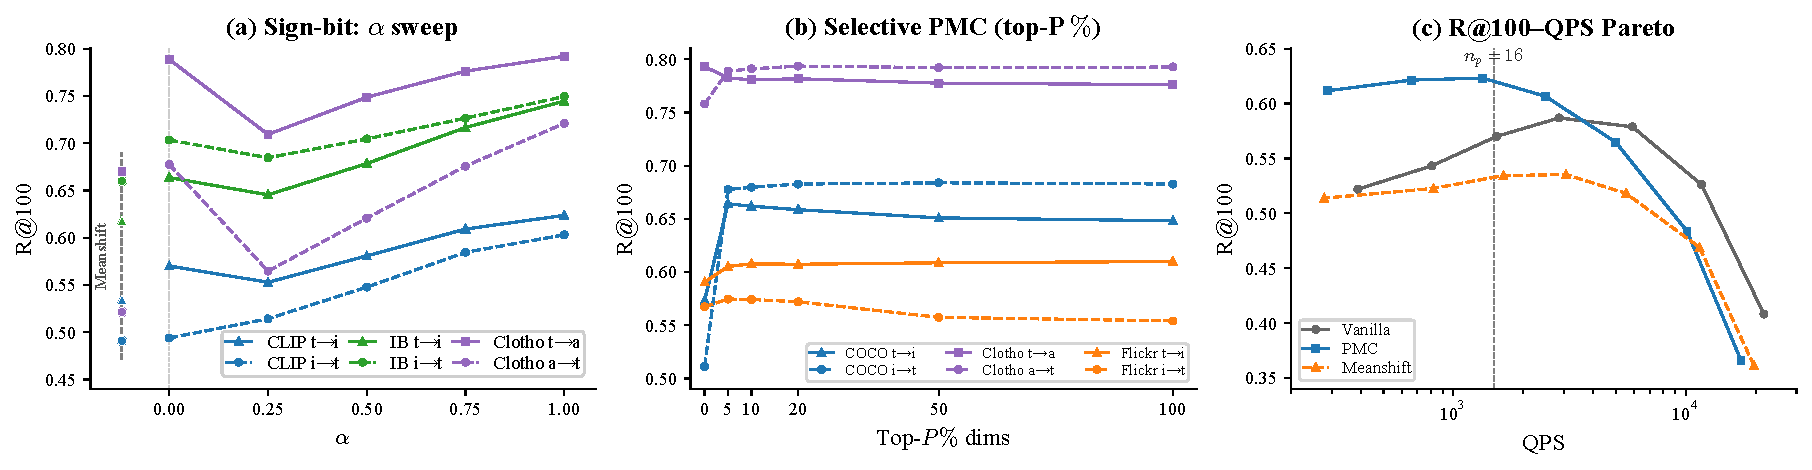
\includegraphics[width=\linewidth]{figures/fig3_analysis.pdf}
  \Description{Three-panel analysis figure. Panel (a) shows BQ alpha sweep curves on MSCOCO and Clotho with mean shift markers and best performance near alpha equals 1. Panel (b) shows selective PMC versus top-P percent dimensions. Panel (c) shows R@100 versus QPS Pareto curves in log-scale where PMC dominates Vanilla at comparable throughput.}
  \caption{(a) BQ R@100 vs.\ shift strength $\alpha$ on MSCOCO+Clotho ($\alpha{=}0$: MeanShift, $\alpha{=}1$: full DB-side PMC): $\alpha{=}1$ is best or near-best, justifying the default. (b) Selective PMC: on concentrated-gap MSCOCO, top-$P{=}5$\% already reaches peak R@100; diffuse gaps require broader correction. (c) R@100--QPS Pareto: PMC dominates Vanilla across throughput levels.}\label{fig:analysis-bcd}
\end{figure*}

\section{Method}\label{sec:method}

\subsection{Problem Setup}\label{sec:setup}

Let $\phi$ be a frozen multimodal encoder mapping inputs from modalities $a$
and $b$ into $\mathbb{R}^d$.
The database $\mathcal{X} = \{\phi(x_i)\}$ consists of modality-$b$ embeddings;
queries $q = \phi(q_j)$ come from modality~$a$.
We denote the per-modality means $\boldsymbol{\mu}_q = \mathbb{E}[\phi(q)]$
and $\boldsymbol{\mu}_x = \mathbb{E}[\phi(x)]$,
and the \emph{modality gap} $\mathbf{g} = \boldsymbol{\mu}_q - \boldsymbol{\mu}_x$.
The goal is to build a compressed ANN index over $\mathcal{X}$ that answers
cross-modal queries with high recall under a fixed memory budget.

\subsection{BQ Vulnerability to Modality Gap}\label{sec:why}

BQ encodes each dimension as $\hat{x}_i = \mathrm{sign}(x_i - c_i)$ relative to centroid $c$, as in RaBitQ~\cite{gao2024rabitq} and BBQ (Apache Lucene). With one bit, the decision boundary passes exactly through $c$ with \emph{zero error margin}.
Let $\delta_i = x_i - c_i$ be the residual under $c = \boldsymbol{\mu}_x$ (so $b_i = \mathrm{sign}\,\delta_i$); shifting to $c^* = \boldsymbol{\mu}_x + \alpha\mathbf{g}$ flips dimension~$i$'s sign iff
\begin{equation}\label{eq:ratio-form}
  \delta_i(\delta_i - \alpha g_i) < 0\,,\quad\text{i.e.,}\quad 0 < \frac{\delta_i}{\alpha g_i} < 1\,.
\end{equation}
Under smooth symmetric residual densities $p_i$ near the decision boundary, a first-order expansion yields the expected number of flips:
\begin{equation}\label{eq:expected-flips}
  \mathbb{E}[F]\;\approx\;\alpha\sum_i p_i(0)\,|g_i|\,,
\end{equation}
a density-weighted $\ell_1$ norm of the gap. Eq.~\eqref{eq:ratio-form} shows that flip risk in dimension~$i$ grows with $|\alpha g_i|/|\delta_i|$: larger gap components produce wider flip intervals. When gap energy is concentrated---in CLIP-L on MSCOCO, top 10\% of dimensions carry ${\approx}90$\% of $\|\mathbf{g}\|^2$---corruption is \emph{structured} rather than random, biasing Hamming distance estimates systematically. The same offset misaligns IVF cluster assignments, compounding routing errors with code corruption. Eq.~\eqref{eq:expected-flips} formalizes this scaling, explaining the gap-proportional gains in Table~\ref{tab:main} and why top-5\% selective PMC already reaches peak recall (Figure~\ref{fig:analysis-bcd}b).
Multi-bit quantization (IVFPQ~\cite{jegou2011pq}, OPQ~\cite{ge2013opq}) partially absorbs displacement through wider error margins; BQ is maximally vulnerable and is the focus of our main claims (multi-bit: Section~\ref{sec:multibit}). PMC applies to all $\mathrm{sign}(\cdot{-}c)$ methods (BinaryFlat, BinaryIVF, BBQ, RaBitQ) and analogous schemes such as LSH~\cite{wang2018hashsurvey}.\looseness=-1

\subsection{PMC Correction}\label{sec:pmc}

PMC applies a one-time centroid alignment \emph{before} index
construction.
Given a training sample of queries from modality~$a$ and the database from
modality~$b$, we compute the gap $\mathbf{g}$ and shift database vectors
toward the query centroid:
%
\begin{equation}\label{eq:pmc}
  \mathbf{x}' = \frac{\mathbf{x} + \alpha \, \mathbf{g}}
                      {\|\mathbf{x} + \alpha \, \mathbf{g}\|}
  \,,\qquad
  \mathbf{q}' = \frac{\mathbf{q} - (1-\alpha) \, \mathbf{g}}
                      {\|\mathbf{q} - (1-\alpha) \, \mathbf{g}\|}
\end{equation}
%
where $\alpha \in [0,1]$ interpolates between full query-side correction
($\alpha{=}0$, equivalent to mean shift) and full database-side alignment
($\alpha{=}1$).
The BQ index is then built on $\{\mathbf{x}'\}$; in our main setting
$\alpha{=}1$ (full database-side alignment), query-time transformation is
identity ($\mathbf{q}'{=}\mathbf{q}$), so serving incurs no extra cost.

\textbf{Effectiveness of {\boldmath$\alpha{=}1$}.}
Per-vector renormalization after the shift preserves unit-norm structure; the $\alpha$-sweep in Figure~\ref{fig:analysis-bcd}a confirms $\alpha{=}1$ as best or near-best across all tested settings.\looseness=-1

\textbf{Selective PMC as a mechanism test.}
We restrict correction to top-$P$\% dimensions ranked by $|g_i|$:
\begin{align}
  g_{\mathrm{sel},i} &= \begin{cases}
    g_i & \text{if } |g_i| \ge |g|_{(P)} \\
    0   & \text{otherwise}
  \end{cases} \label{eq:selective-gap} \\[2pt]
  \mathbf{x}'_{\mathrm{sel}} &= \frac{\mathbf{x} + \alpha \, \mathbf{g}_{\mathrm{sel}}}{\|\mathbf{x} + \alpha \, \mathbf{g}_{\mathrm{sel}}\|} \label{eq:selective}
\end{align}
where $|g|_{(P)}$ is the top-$P$\% magnitude threshold on $|g_i|$. The cumulative energy captured by $\mathbf{g}_{\mathrm{sel}}$ is
\begin{equation}\label{eq:energy-frac}
  \mathcal{E}(P) = \frac{\sum_{i \in \mathcal{S}_P} g_i^2}{\|\mathbf{g}\|^2}\,,
  \quad \mathcal{S}_P = \bigl\{i : |g_i| \geq |g|_{(P)}\bigr\}\,.
\end{equation}
Since flip risk concentrates in high-$|g_i|$ dimensions (Eq.~\eqref{eq:ratio-form}), correcting only the highest-energy ones suffices: for CLIP the top 10\% by $|g_i|$ carry 86--92\% of total gap energy across all tested datasets, so $P{=}5$\% already recovers peak recall; ImageBind's diffuse gap (${\approx}72\%$) requires full-vector correction.\looseness=-1


\section{Experiments}\label{sec:experiments}

\subsection{Setup}\label{sec:exp-setup}

We evaluate three frozen backbones---CLIP ViT-B/32 ($d{=}512$)~\cite{radford2021clip}, CLIP ViT-L/14 ($d{=}768$), ImageBind ($d{=}1024$)~\cite{girdhar2023imagebind}---on image--text and audio--text retrieval: MSCOCO 5K~\cite{lin2014coco}, Flickr30K ($n{=}31$K)~\cite{young2014flickr30k}, AudioCaps~\cite{kim2019audiocaps} (884 clips, 4{,}415 captions; audio DB), Clotho v2 ($n{=}5{,}926$)~\cite{drossos2020clotho}, and LAION-400M (407M vectors, 410 shards; exact inner-product (IP) ground truth for 10K random queries per direction via per-shard IndexFlatIP merged into a global top-100---a full-corpus brute-force scan)~\cite{schuhmann2021laion}. Indexes use FAISS~\cite{johnson2021faiss,douze2024faiss}: IVFRaBitQFastScan (1-bit, 33--136\,B/vec) and IVFPQ/OPQ~\cite{jegou2011pq,ge2013opq} ($m{=}16$, 64\,B/vec); per FAISS's IVF heuristic, $n_\mathrm{list}{=}\lceil\sqrt{n}\,\rceil$ and $n_\mathrm{probe}{\approx}n_\mathrm{list}/4$, matched across methods; with reranking (Sec.~\ref{sec:rerank}) we set $n_\mathrm{probe}{\approx}n_\mathrm{list}$ and exact-rerank the top $K'{=}400$; LAION uses $n_\mathrm{list}{=}80\mathrm{K}{\approx}4\sqrt{N}$, $n_\mathrm{probe}{=}256$, 30.4\,GB at 72\,B/vec ($28\times$); PMC leaves bytes/vector identical to Vanilla; BQ baselines: BinaryFlat, BinaryIVF, rotated BinaryFlat (BBQ-style). We report R@100 against exact-IP ground truth on original (unshifted) embeddings, except AudioCaps, which uses standard caption annotations (one clip per caption; that clip's captions in reverse)---PMC modifies only the index-internal representation (analogous to OPQ rotation), so gains reflect better approximation, not redefined relevance---and QPS (queries per second) as the single-threaded median over 5 runs. All runs use a single Intel Core i7-12700F, 32\,GB RAM, CPU-only.\looseness=-1

\begin{table}[t]
\caption{R@10 at the no-reranking operating points of Table~\ref{tab:mainresults}. Each cell Vanilla\,/\,MeanShift\,/\,PMC; \textbf{bold}\,=\,best per cell.}\label{tab:r10}
\centering
{\footnotesize
\begin{tabular*}{\columnwidth}{@{\extracolsep{\fill}}ll cc@{}}
\toprule
\textbf{Dataset} & \textbf{Enc.} & $q{\to}db$ & $db{\to}q$ \\
\midrule
MSCOCO     & CLIP & .40\,/\,.38\,/\,\textbf{.46} & .29\,/\,.30\,/\,\textbf{.39} \\
           & CL-L & .36\,/\,.37\,/\,\textbf{.48} & .26\,/\,.35\,/\,\textbf{.44} \\
           & IB   & .55\,/\,.51\,/\,\textbf{.63} & .57\,/\,.54\,/\,\textbf{.64} \\
Flickr30K  & CL-L & .31\,/\,.26\,/\,\textbf{.38} & .22\,/\,.29\,/\,\textbf{.38} \\
Clotho     & IB   & .59\,/\,.45\,/\,\textbf{.60} & .48\,/\,.35\,/\,\textbf{.54} \\
AudioCaps  & IB   & .39\,/\,.43\,/\,\textbf{.44} & .44\,/\,.46\,/\,\textbf{.48} \\
LAION-400M & CLIP & .075\,/\,.038\,/\,\textbf{.086} & .035\,/\,.028\,/\,\textbf{.048} \\
\bottomrule
\end{tabular*}}
\end{table}

\begin{table}[t]
\caption{Mechanism/control checks ($\alpha{=}1$). $J@100$: top-100 Jaccard vs.\ exact-IP GT; cos@25: calibration cosine at $n_\mathrm{calib}{=}25$.}\label{tab:mechanism}
\centering
{\footnotesize
\begin{tabular*}{\columnwidth}{@{\extracolsep{\fill}}lcccc@{}}
\toprule
\textbf{Direction} & \textbf{Flip\%} & \textbf{$J@100$} & \textbf{BinaryFlat R@100} & \textbf{cos@25} \\
\midrule
MSCOCO t$\to$i    & 16.14 & .585 & .507\,$\to$\,.570 & .986 \\
MSCOCO i$\to$t    & 15.99 & .542 & .458\,$\to$\,.568 & .986 \\
AudioCaps t$\to$a & 14.34 & .801 & .630\,$\to$\,.660 & .971 \\
AudioCaps a$\to$t & 17.84 & .799 & .514\,$\to$\,.644 & .955 \\
\bottomrule
\end{tabular*}%
}
\end{table}

\begin{table}[t]
\caption{MSCOCO/CLIP-B/32: component ablation and IVF-RaBitQ controls. Rand/Shuf are mean$\pm$std over 5 seeds.}\label{tab:mech_extra}
\centering
{\footnotesize
\begin{tabular*}{\columnwidth}{@{\extracolsep{\fill}}llcccc@{}}
\toprule
\multicolumn{6}{@{}l}{\textbf{Component ablation}}\\
\textbf{Index} & \textbf{Dir.} & \textbf{Van.} & \textbf{Q-only} & \textbf{DB-only} & \textbf{Both} \\
\midrule
BinaryFlat & t$\to$i & .507 & .569 & \textbf{.570} & \textbf{.570} \\
BinaryFlat & i$\to$t & .458 & \textbf{.571} & .568 & .569 \\
IVF-RaBitQ & t$\to$i & .578 & .541 & \textbf{.637} & .599 \\
IVF-RaBitQ & i$\to$t & .515 & .495 & \textbf{.608} & .554 \\
\bottomrule
\end{tabular*}\\[0pt]
\begin{tabular*}{\columnwidth}{@{\extracolsep{\fill}}lcccccc@{}}
\toprule
\multicolumn{7}{@{}l}{\textbf{IVF-RaBitQ controls}}\\
\textbf{Dir.} & \textbf{Van.} & \textbf{DB-PMC} & \textbf{Rand} & \textbf{Shuf} & \textbf{S-Flip} & \textbf{NoNorm} \\
\midrule
t$\to$i & .578 & \textbf{.637} & .562$\pm$.009 & .552$\pm$.006 & .514 & .555 \\
i$\to$t & .515 & \textbf{.608} & .564$\pm$.009 & .559$\pm$.009 & .491 & .520 \\
\bottomrule
\end{tabular*}%
}
\end{table}

%% ---------------------------------------------------------------
\subsection{Main Results}\label{sec:results}
%% ---------------------------------------------------------------

PMC improves RaBitQ recall in nearly all tested configurations, with gains scaling with gap magnitude (Table~\ref{tab:mainresults}): Flickr30K i$\to$t reaches $+$45\% and MSCOCO CLIP-L i$\to$t $+$34\%. MeanShift can hurt---it leaves IVF centroids misaligned, degrading routing---while PMC improves or matches both directions. Across all 16 BQ method $\times$ direction configurations, PMC improves or matches R@100 without exception (Table~\ref{tab:signbit_methods}); the same ordering holds at R@10, where PMC is best in all 14 dataset $\times$ direction configurations (Table~\ref{tab:r10}), so the gain is not confined to deep result lists. RotatedBinary suffers most---rotation spreads the concentrated gap energy across all bits---and gains most from PMC.
PMC adds no per-query work, so QPS tracks Vanilla across all $n_\mathrm{probe}$ (Figure~\ref{fig:analysis-bcd}c).\looseness=-1

\textbf{{\boldmath$\|\mathbf{g}\|$} as predictor.}
The ratio condition~\eqref{eq:ratio-form} implies more flips at higher gap, and R@100 gains track $\|\mathbf{g}\|$: MSCOCO CL-L ($\|\mathbf{g}\|{=}.82$) and Flickr30K CL-L ($\|\mathbf{g}\|{=}.77$) show the largest gains, whereas AudioCaps ($\|\mathbf{g}\|{=}.61$) gains only marginally---its gap is small relative to intra-class variance. Direct bit-level checks corroborate this (Table~\ref{tab:mechanism}): PMC induces 14--18\% sign-bit flips while preserving nontrivial ground-truth top-100 overlap ($J@100{=}0.54$--$0.80$) and repairs BinaryFlat R@100 in every direction.\looseness=-1

At 407M-vector deployment scale, LAION-400M ($\|\mathbf{g}\|{=}.72$) confirms the gap-proportional pattern in both directions (Table~\ref{tab:mainresults}).\looseness=-1

%% ---------------------------------------------------------------
\subsection{Robustness under Exact Reranking}\label{sec:rerank}
%% ---------------------------------------------------------------

With reranking~\cite{wang2011cascade} we exact-rescore the top-$K'$ candidates (Sec.~\ref{sec:exp-setup}; identical per-method budget). Vanilla's no-rerank recall is capped by what its corrupted codes admit; PMC repairs the pool and carries this lead into reranking, improving or matching Vanilla and MeanShift in every cell except LAION-400M reverse across $K'\in\{100,200,400,500\}$ (MSCOCO t$\to$i PMC .62/.80/.90/.93 vs.\ Vanilla .53/.69/.81/.85; Table~\ref{tab:mainresults} reports $K'{=}400$), reaching $R@100{\geq}0.90$ at a smaller budget. There, exact rescoring lets Vanilla overtake PMC at $K'{\geq}200$---a scan-depth effect: LAION probes only $0.32\%$ of its lists ($n_\mathrm{probe}{=}256$), so PMC's flatter pool covers fewer true positives, whereas small corpora rerank near-exhaustively.

%% ---------------------------------------------------------------
\subsection{Ablation Study}\label{sec:ablation}
%% ---------------------------------------------------------------

\begin{table}[t]
\caption{PMC generality on IVFPQ and OPQ across encoders (R@100 Vanilla\,/\,\textbf{PMC}, mean over both directions; per-direction omitted).}\label{tab:multibit}
\centering
{\footnotesize
\begin{tabular*}{\columnwidth}{@{\extracolsep{\fill}}ll cccc@{}}
\toprule
\textbf{Dataset} & \textbf{Enc.} & \multicolumn{2}{c}{\textbf{IVFPQ}} & \multicolumn{2}{c}{\textbf{OPQ}} \\
\cmidrule(lr){3-4}\cmidrule(lr){5-6}
& & R@100 & $\Delta$ & R@100 & $\Delta$ \\
\midrule
MSCOCO & CLIP & .52\,/\,\textbf{.64} & +23\% & .64\,/\,\textbf{.67} & +4\% \\
       & CL-L & .39\,/\,\textbf{.61} & +56\% & .57\,/\,\textbf{.67} & +17\% \\
       & IB   & .59\,/\,\textbf{.69} & +17\% & .70\,/\,\textbf{.77} & +9\% \\
Flickr & CL-L & .47\,/\,\textbf{.50} & +7\% & .51\,/\,\textbf{.52} & +1\% \\
\bottomrule
\end{tabular*}%
}

\end{table}

Calibration is stable from $n_\mathrm{calib}{=}25$ (cosine $0.955$--$0.986$ across modalities, Table~\ref{tab:mechanism}; R@100 flat within .003 up to $n_\mathrm{calib}{=}400$), making PMC practical with few cross-modal samples. BinaryFlat is insensitive to shift direction, but IVF-RaBitQ strongly prefers DB-only correction (.637/.608) over Q-only (.541/.495) or both sides (.599/.554)---shifting both re-displaces the routing pivot, confirming the centroid must be corrected at the source, where it is both routing pivot and code boundary. Four controls (random, shuffled, sign-flipped, un-normalized shift) all trail DB-PMC (Table~\ref{tab:mech_extra}), ruling out arbitrary perturbation.\looseness=-1

%% ---------------------------------------------------------------
\subsection{Multi-Bit Generality}\label{sec:multibit}
%% ---------------------------------------------------------------

{\emergencystretch=1em PMC generalizes beyond 1-bit: averaged over both directions it improves IVFPQ and OPQ across all encoders and datasets (audio omitted; $n_\mathrm{db}$ too small for codebook training), with the gap-proportional trend persisting (Table~\ref{tab:multibit}). OPQ's learned rotation partly absorbs the shift, giving smaller but complementary gains; IVFPQ lacks this and benefits more.\looseness=-1\par}

\section{Conclusion}\label{sec:conclusion}

PMC addresses cross-modal centroid mismatch in compressed ANN through a build-time database-side correction that rewrites the index's routing pivots and sign-bit boundaries rather than shifting only queries, yielding recall gains that scale with modality-gap magnitude at no extra index memory and, at $\alpha{=}1$, no serving-time query transform; the lone regime favoring uncorrected codes---deep reranking under sub-1\% list probing at 400M scale---is a scan-depth effect, not a limit of the correction. Future work: drift-adaptive $\alpha$ for streaming, graph-based ANN, and billion-scale deployment.


\section*{GenAI Usage Disclosure}
Generative AI tools (Claude) were used for code scaffolding and LaTeX formatting.
All experimental design, results, analyses, and scientific claims were
independently produced and verified by the authors.

\balance
\emergencystretch=2em
\bibliographystyle{ACM-Reference-Format}
\bibliography{refs}

\end{document}
